\documentclass[10pt,twocolumn]{article}
\usepackage[a4paper,margin=1.75cm,columnsep=0.65cm]{geometry}
\usepackage[T1]{fontenc}
\usepackage{lmodern}
\usepackage{microtype}
\usepackage{graphicx}
\usepackage{booktabs}
\usepackage{tikz}
\usetikzlibrary{arrows.meta,positioning,shapes.misc,fit,backgrounds}
\usepackage[font=footnotesize,labelfont=bf,skip=3pt]{caption}
\usepackage{float}
\usepackage[hidelinks]{hyperref}
\setlength{\parskip}{0pt}
\raggedbottom
\setlength{\textfloatsep}{8pt}
\setlength{\intextsep}{6pt}
\graphicspath{{image/}}

\title{\vspace{-1.2em}Simulation-Derived 5G/UAS Cyber-Incident Telemetry:\\Co-Simulation Setup and Experiment\vspace{-0.3em}}
\author{Basudeo Shrestha}
\date{\vspace{-1.5em}}

\begin{document}
\maketitle

\begin{abstract}
\noindent A co-simulation pipeline produces labelled network telemetry for
cyber-incident detection in an uncrewed aircraft system (UAS) on a 5G
network. A PX4 software-in-the-loop (SITL) autopilot flies a drone in Gazebo,
the Robot Operating System 2 (ROS~2) records it through MAVROS, and the
recorded pose drives a user equipment (UE) in Simu5G on OMNeT++ and INET. A
bridge maps the network output to the 44-column schema of an existing
synthetic dataset, one row per flow per window, with labels applied from a
manifest after every measurement. A 43-run matrix of benign, suspicious and
malicious scenarios yields 17,779 rows; every run shows its predicted effect
and a leakage audit reproduces every flag from behaviour alone. Gradient
boosting reaches macro-F1 0.82, a random forest 0.79 and logistic regression
0.58, against 0.99 or better on the synthetic reference; the gap lies in
suspicious windows close to benign traffic, the realism the pipeline was
built to add.
\end{abstract}

\noindent\textbf{Keywords:} UAS, 5G, co-simulation, Gazebo, PX4, ROS~2,
Simu5G, OMNeT++, network telemetry, cyber-incident detection, dataset
generation, leakage control.

\section{Methodology}

The work builds a small co-simulator that produces a validated cyber-incident
telemetry dataset for unmanned aerial systems over a modelled 5G network.
Every value is measured from a simulation output; the scenario manifest
supplies only the labels, after the measurements are taken. A setup stage
built the simulator and produced an eight-run dataset, one benign, one
suspicious and one per attack class; the experiment stage ran a 43-run matrix
for a controlled comparison with a synthetic reference of the same 44-column
schema.

\subsection{Architecture}

Figure~\ref{fig:arch} shows the three layers. The \emph{flight layer} is
Gazebo Sim 8.11 with a PX4 SITL quadrotor (x500) flying a waypoint route in a
Baylands-style world, exposed to ROS~2 Jazzy through MAVROS. The
\emph{network layer} is OMNeT++~6.0.1 with INET~4.5 and Simu5G~1.2.2: one
NR gNodeB, a 5G core (UPF and intermediate UPF), an edge node and a mission
backend host; the drone is an NR user equipment whose mobility replays the
recorded flight. The \emph{bridge} joins the two on a shared clock: it
writes one row per flow per aggregation window and applies the manifest's
label windows after every measurement. All components run on one
Ubuntu~24.04 machine.

\begin{figure}[H]
\centering
\resizebox{\columnwidth}{!}{%
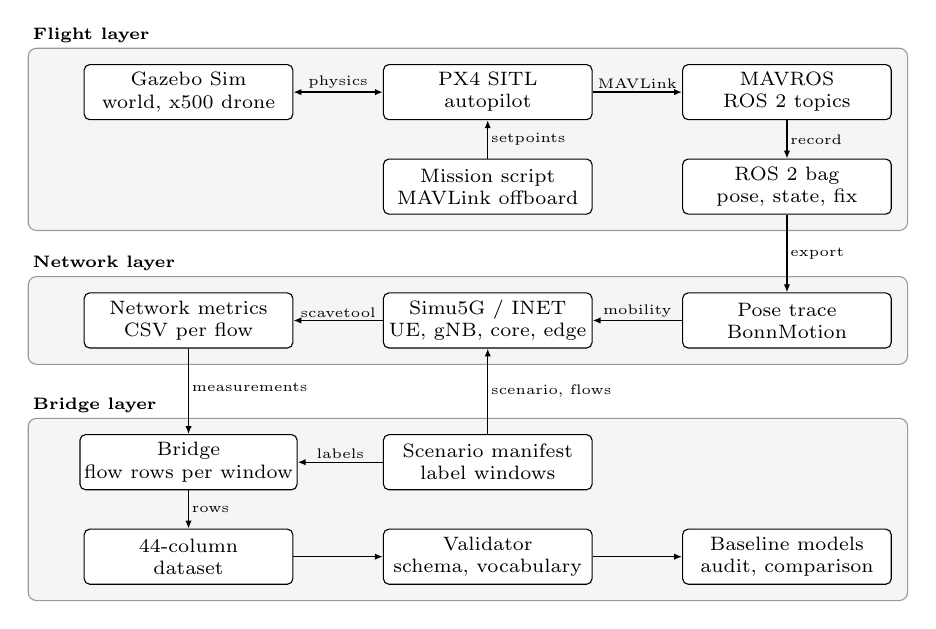
\begin{tikzpicture}[x=1mm, y=1mm, font=\scriptsize,
  box/.style={draw, rounded corners=2pt, fill=white, minimum width=26.5mm, minimum height=7mm, inner sep=1.5pt, align=center},
  arr/.style={-{Latex[length=1mm, width=0.8mm]}, line width=0.5pt},
  lab/.style={font=\fontsize{4.6}{5}\selectfont, inner sep=1pt, text=black},
  band/.style={draw=black!40, rounded corners=3pt, fill=black!4, inner sep=2mm},
  title/.style={font=\fontsize{6.5}{7}\selectfont\bfseries, text=black, inner sep=0pt, anchor=south west}]
  % flight layer
  \node[box] (gz)  at (0,0)    {Gazebo Sim\\world, x500 drone};
  \node[box] (px4) at (38,0)   {PX4 SITL\\autopilot};
  \node[box] (mav) at (76,0)   {MAVROS\\ROS 2 topics};
  \node[box] (mis) at (38,-12) {Mission script\\MAVLink offboard};
  \node[box] (bag) at (76,-12) {ROS 2 bag\\pose, state, fix};
  % network layer
  \node[box] (trc) at (76,-29) {Pose trace\\BonnMotion};
  \node[box] (s5g) at (38,-29) {Simu5G / INET\\UE, gNB, core, edge};
  \node[box] (net) at (0,-29)  {Network metrics\\CSV per flow};
  % bridge and outputs
  \node[box] (br)  at (0,-47)  {Bridge\\flow rows per window};
  \node[box] (man) at (38,-47) {Scenario manifest\\label windows};
  \node[box] (ds)  at (0,-59)  {44-column\\dataset};
  \node[box] (val) at (38,-59) {Validator\\schema, vocabulary};
  \node[box] (mdl) at (76,-59) {Baseline models\\audit, comparison};
  \begin{scope}[on background layer]
    \coordinate (L) at ([xshift=-4.5mm]br.west);
    \node[band, fit=(L |- gz.north)(mdl.east |- mis.south)] (fl) {};
    \node[band, fit=(L |- net.north)(mdl.east |- net.south)] (nl) {};
    \node[band, fit=(L |- br.north)(mdl.east |- ds.south)] (bl) {};
  \end{scope}
  \node[title] at ([xshift=0.6mm, yshift=0.6mm]fl.north west) {Flight layer};
  \node[title] at ([xshift=0.6mm, yshift=0.6mm]nl.north west) {Network layer};
  \node[title] at ([xshift=0.6mm, yshift=0.6mm]bl.north west) {Bridge layer};
  \draw[arr, {Latex[length=1mm, width=0.8mm]}-{Latex[length=1mm, width=0.8mm]}] (gz) -- node[lab, above] {physics} (px4);
  \draw[arr] (px4) -- node[lab, above] {MAVLink} (mav);
  \draw[arr] (mis) -- node[lab, right] {setpoints} (px4);
  \draw[arr] (mav) -- node[lab, right] {record} (bag);
  \draw[arr] (bag) -- node[lab, right] {export} (trc);
  \draw[arr] (trc) -- node[lab, above] {mobility} (s5g);
  \draw[arr] (s5g) -- node[lab, above] {scavetool} (net);
  \draw[arr] (net) -- node[lab, right, pos=0.45] {measurements} (br);
  \draw[arr] (man) -- node[lab, above] {labels} (br);
  \draw[arr] (man) -- node[lab, right] {scenario, flows} (s5g);
  \draw[arr] (br) -- node[lab, right] {rows} (ds);
  \draw[arr] (ds) -- (val);
  \draw[arr] (val) -- (mdl);
\end{tikzpicture}}
\caption{Simulator architecture: flight, network and bridge layers.}
\label{fig:arch}
\end{figure}

\subsection{Data collection pipeline}

Each run follows eight steps (Figure~\ref{fig:pipe}), driven by one YAML
manifest holding the mission settings (speed, duration, drone count,
profile), the network settings (cells, load, slice profile, wireless
condition, seed), the injected event and the label windows. Steps 1 and 2 run
once per flight, 3 to 6 once per run, 7 and 8 once per dataset build.

\begin{figure}[H]
\centering
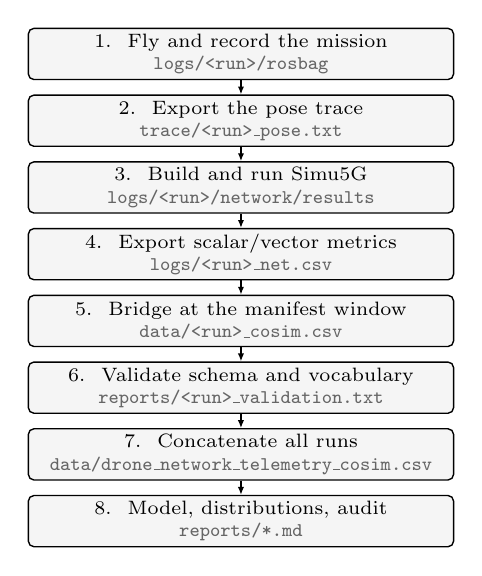
\begin{tikzpicture}[font=\scriptsize, >={Latex[length=1mm, width=0.8mm]}, line width=0.5pt, node distance=1.8mm,
  st/.style={draw, rounded corners=2pt, fill=gray!8, minimum width=54mm, minimum height=6.5mm, inner xsep=4pt, inner ysep=1pt, align=center},
  ou/.style={font=\scriptsize\ttfamily, text=black!60}]
  \node[st] (s1) {1.\; Fly and record the mission\\{\ttfamily\color{black!60}logs/<run>/rosbag}};
  \node[st, below=of s1] (s2) {2.\; Export the pose trace\\{\ttfamily\color{black!60}trace/<run>\_pose.txt}};
  \node[st, below=of s2] (s3) {3.\; Build and run Simu5G\\{\ttfamily\color{black!60}logs/<run>/network/results}};
  \node[st, below=of s3] (s4) {4.\; Export scalar/vector metrics\\{\ttfamily\color{black!60}logs/<run>\_net.csv}};
  \node[st, below=of s4] (s5) {5.\; Bridge at the manifest window\\{\ttfamily\color{black!60}data/<run>\_cosim.csv}};
  \node[st, below=of s5] (s6) {6.\; Validate schema and vocabulary\\{\ttfamily\color{black!60}reports/<run>\_validation.txt}};
  \node[st, below=of s6] (s7) {7.\; Concatenate all runs\\{\ttfamily\color{black!60}data/drone\_network\_telemetry\_cosim.csv}};
  \node[st, below=of s7] (s8) {8.\; Model, distributions, audit\\{\ttfamily\color{black!60}reports/*.md}};
  \foreach \a/\b in {s1/s2,s2/s3,s3/s4,s4/s5,s5/s6,s6/s7,s7/s8} \draw[->] (\a) -- (\b);
\end{tikzpicture}
\caption{The per-run data collection pipeline; each box names the step and the file it produces.}
\label{fig:pipe}
\end{figure}

\paragraph{Flight recording.} Gazebo opens paused; once physics runs,
MAVROS starts, the rates of the three recorded topics are measured, and a
ROS~2 bag opens before the mission arms. The mission script flies PX4 in
offboard mode along the route markers from the world file, patrols for the
manifest duration or hovers, and lands at spawn. The pose topic is exported
as a mobility trace cut at the manifest duration.

\paragraph{Network simulation.} The scenario generator writes the NED
topology and \texttt{omnetpp.ini} for the run: one UE per recorded flight on
its own trace, a 50\,Hz, 76\,B telemetry flow and a 1\,Hz, 200\,B command flow
from the UE to the edge node and backend, plus any injected flow. Cells, X2
links, background load, transmit power and slice profile follow the manifest;
results are exported with \texttt{opp\_scavetool}.

\paragraph{Bridge derivations.} The bridge emits one row per flow per
window. Packet and byte counts come from the edge node's receiver vectors;
latency is the mean frame delay and jitter its standard deviation; loss is
expected minus received over expected, with expected the configured rate
times the window and zero when less than one packet is expected;
retransmission rate is the mean uplink HARQ error rate; signal quality is
$-97$\,dBm plus the mean uplink SINR; the serving-cell vector gives handover
events and counts. The three flags follow from behaviour alone:
\texttt{traffic\_burst\_flag} above three times the highest mission-flow
rate, \texttt{unusual\_destination\_flag} outside the manifest's allowed
set, \texttt{session\_reuse\_flag} when a session identifier reappears from
another source address. Labels are stamped last from the window covering
each row's start time, and a bridge log records window, inputs and row count.

\section{Experiments}
\begin{figure*}[t]
\centering
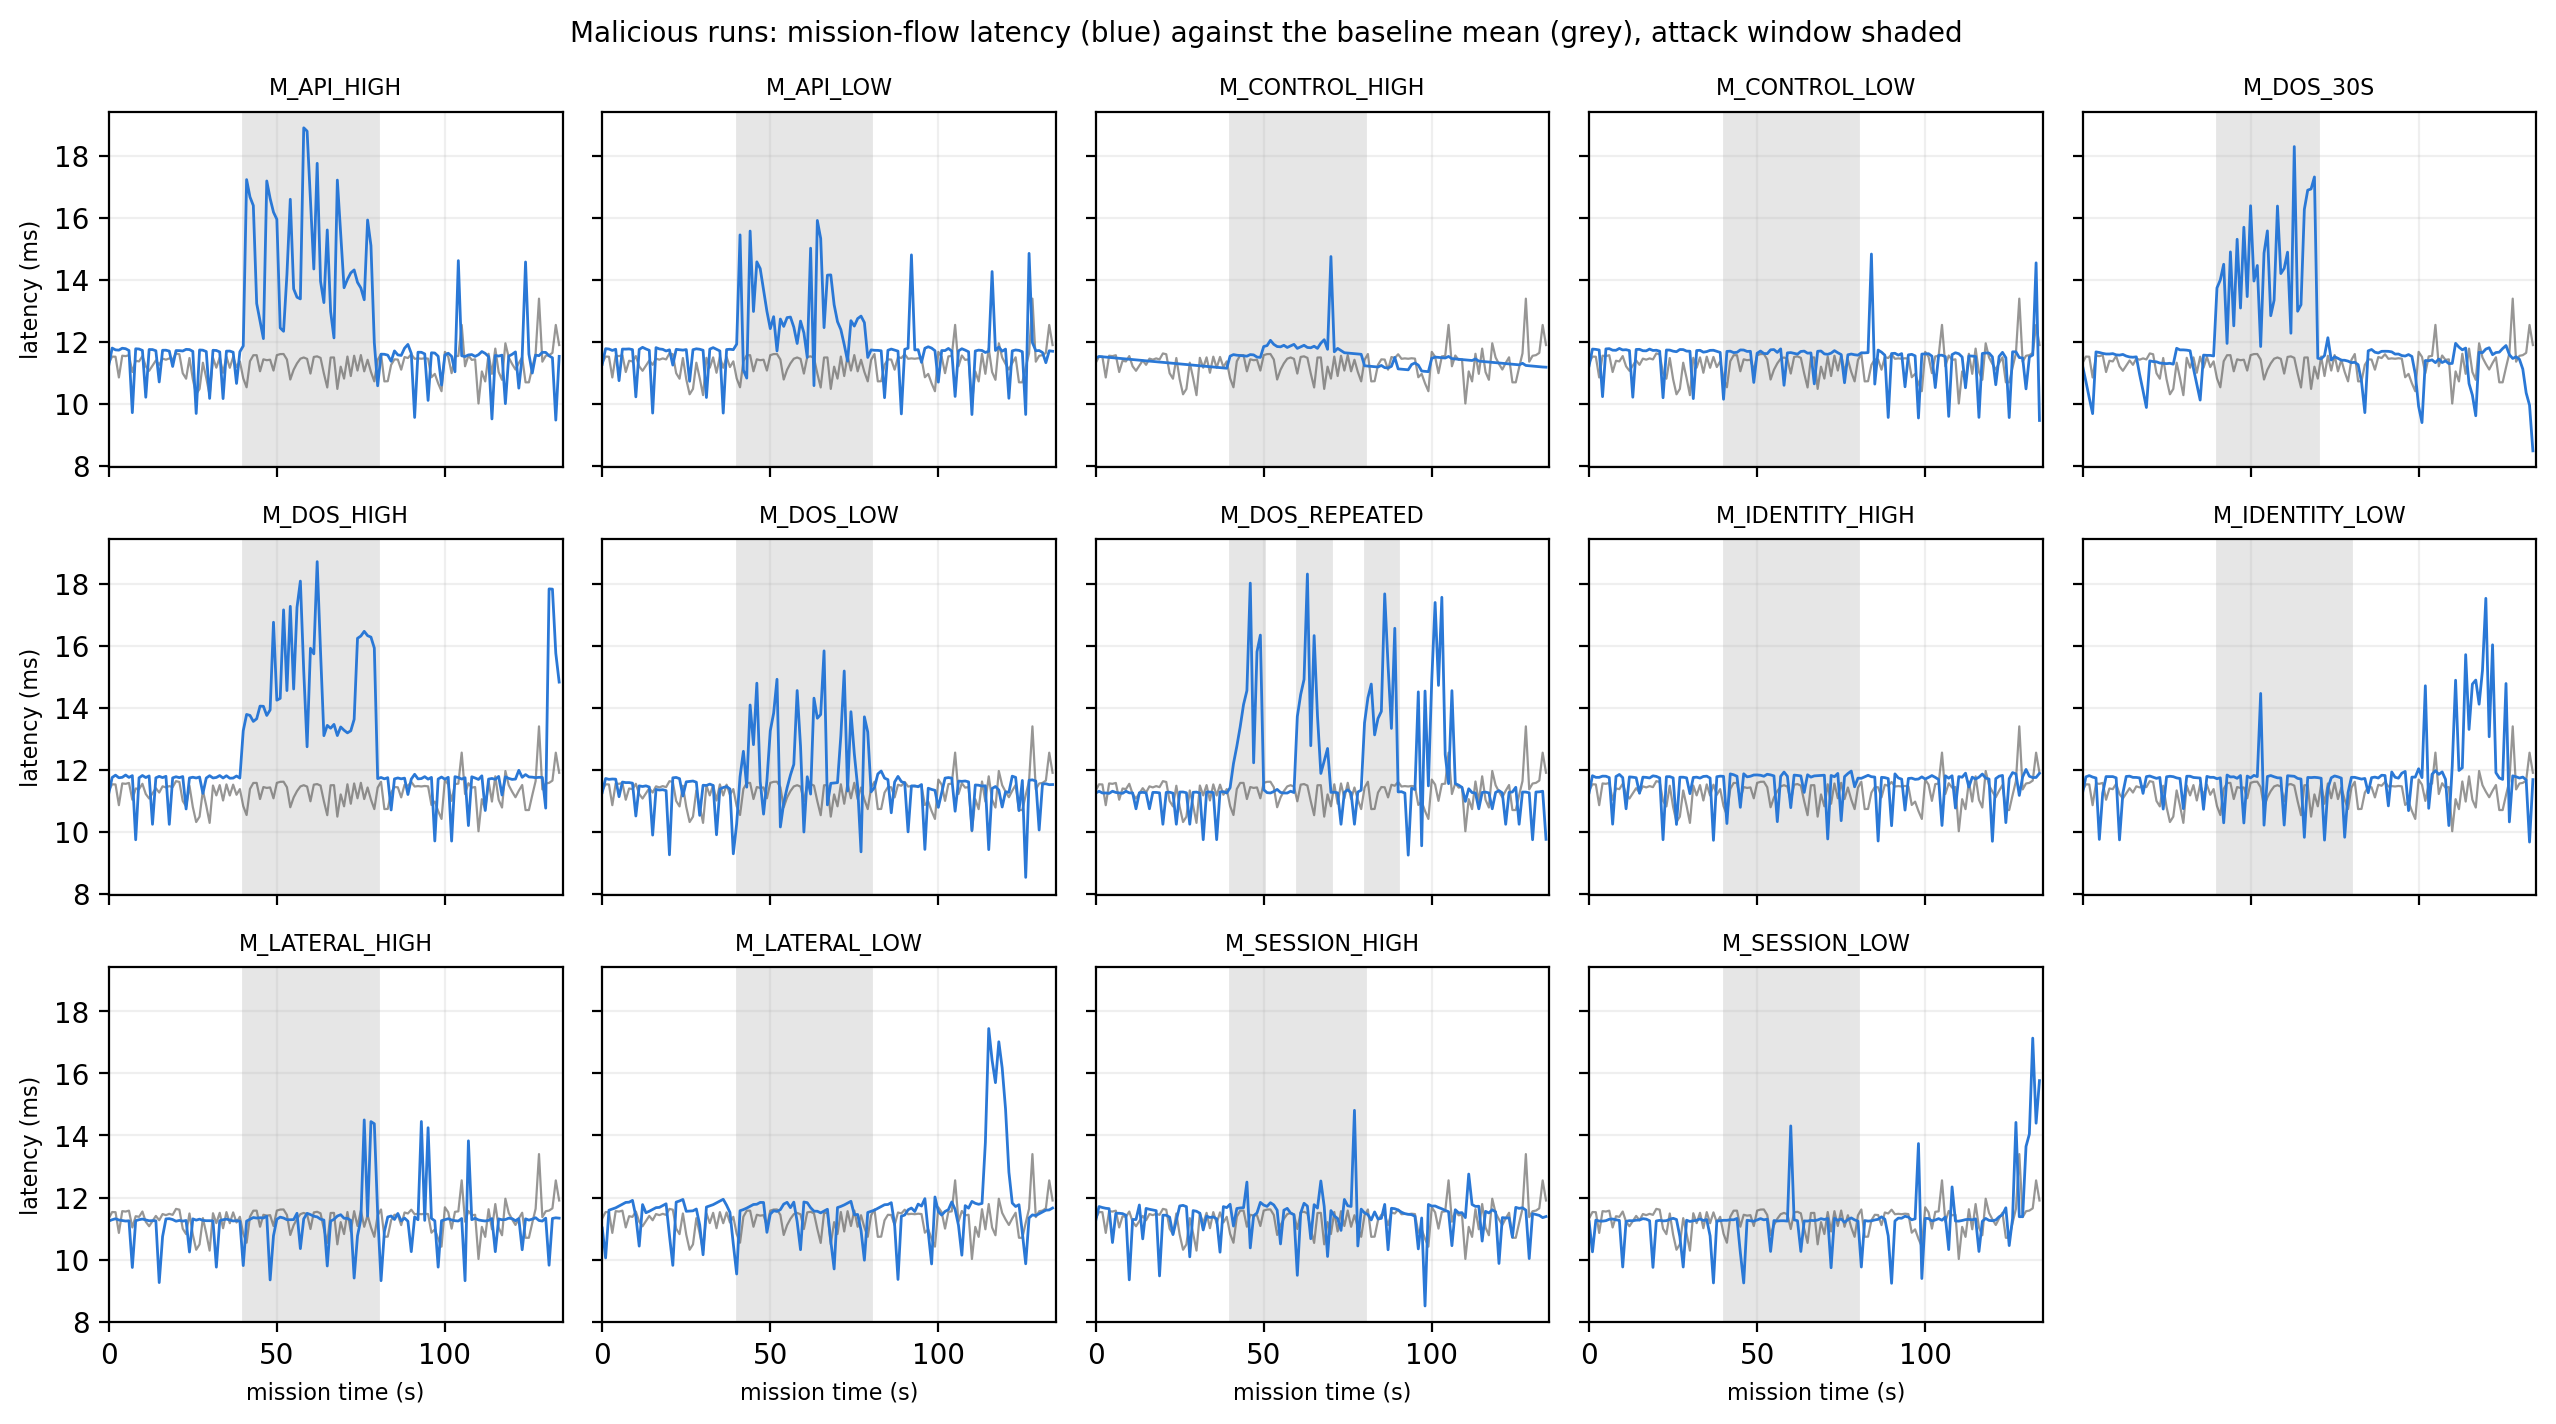
\includegraphics[width=0.68\textwidth]{d2_malicious_panels}
\caption{Malicious runs: mission-flow latency per second (blue) against the mean of the three benign baseline runs (grey); the attack window is shaded.}
\label{fig:panels}
\end{figure*}
\begin{figure*}[t]
\centering
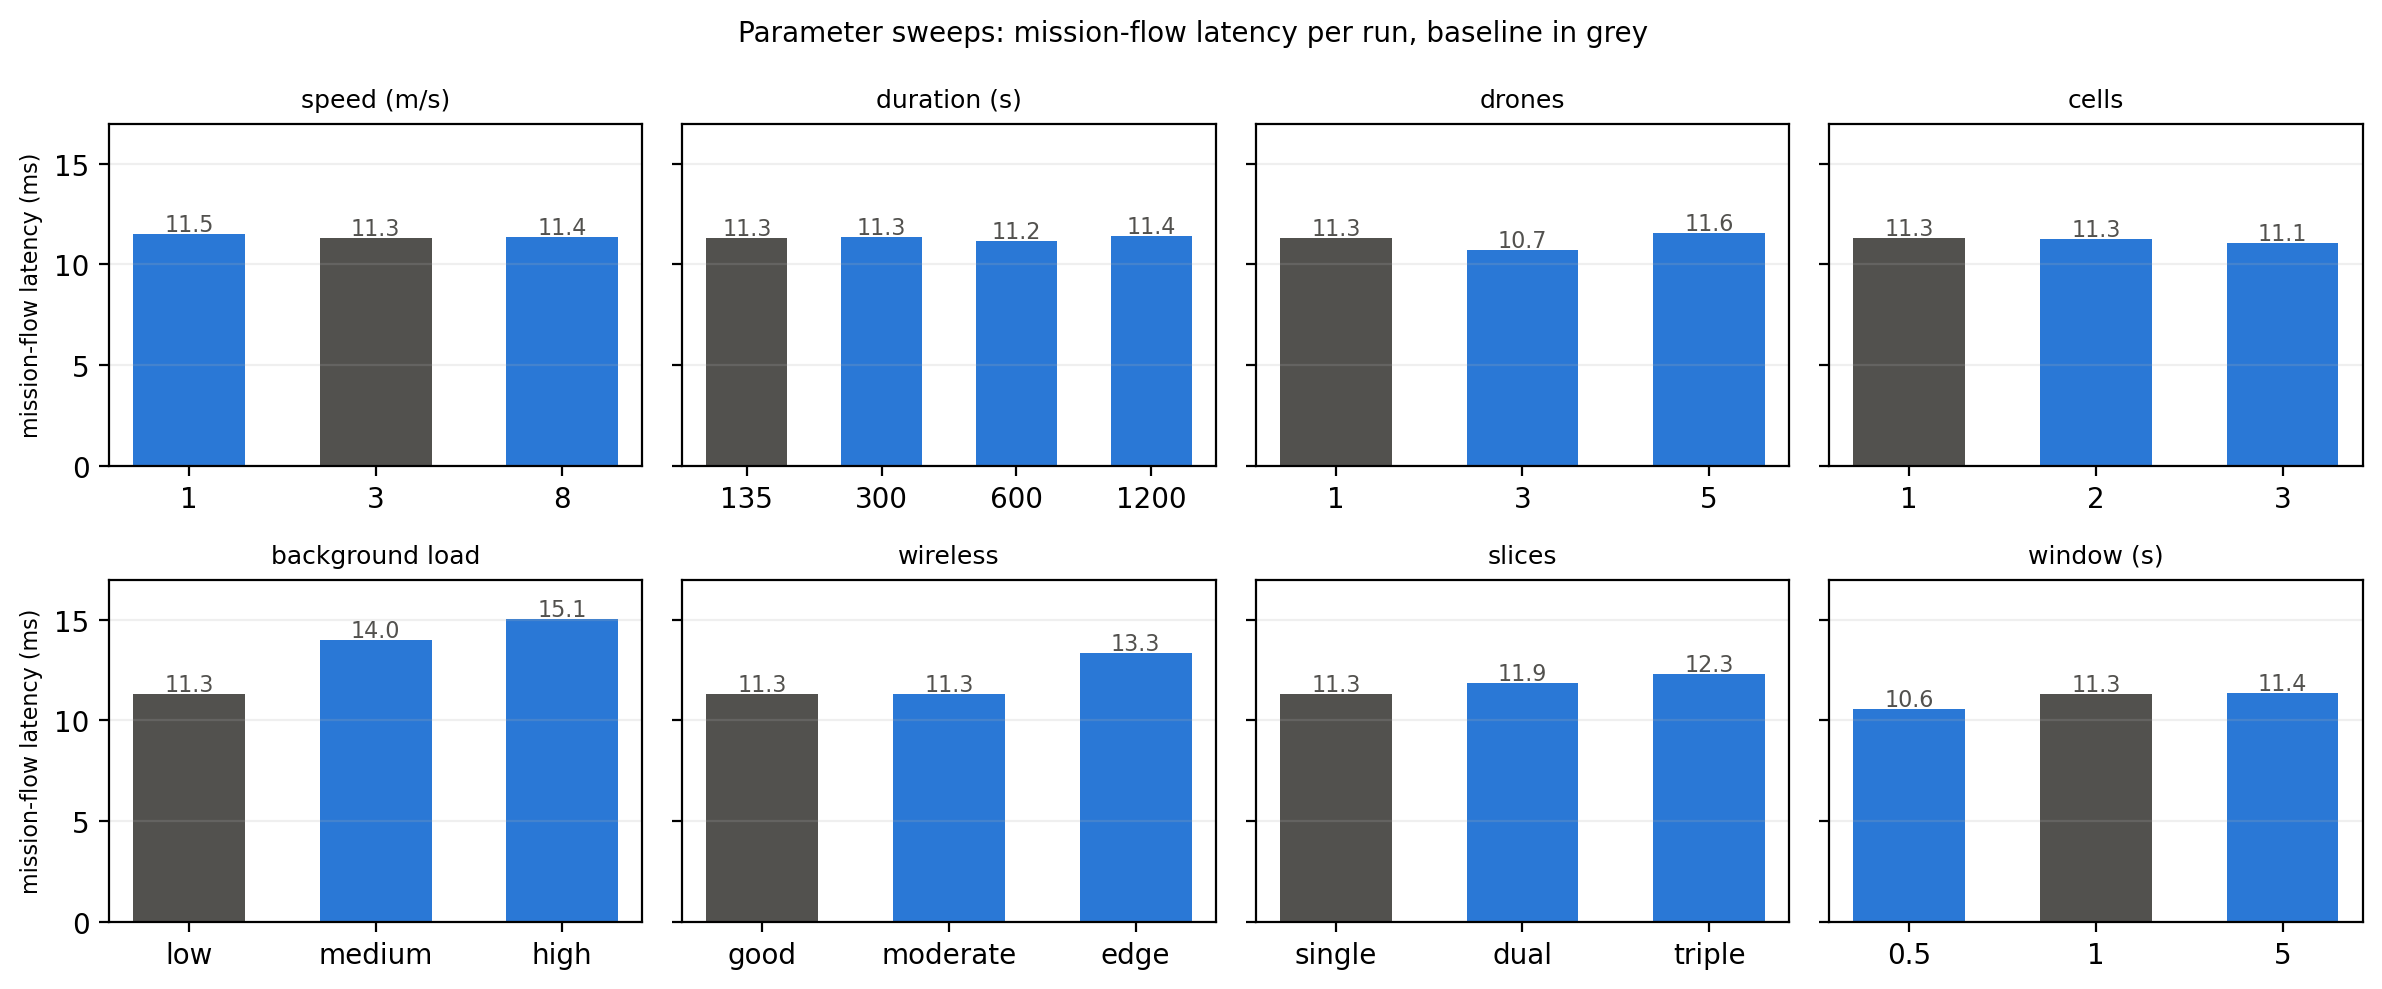
\includegraphics[width=0.50\textwidth]{d2_sweeps}
\caption{Parameter sweeps: mission-flow latency per run, baseline in grey.}
\label{fig:sweeps}
\end{figure*}
\begin{figure*}[t]
\centering
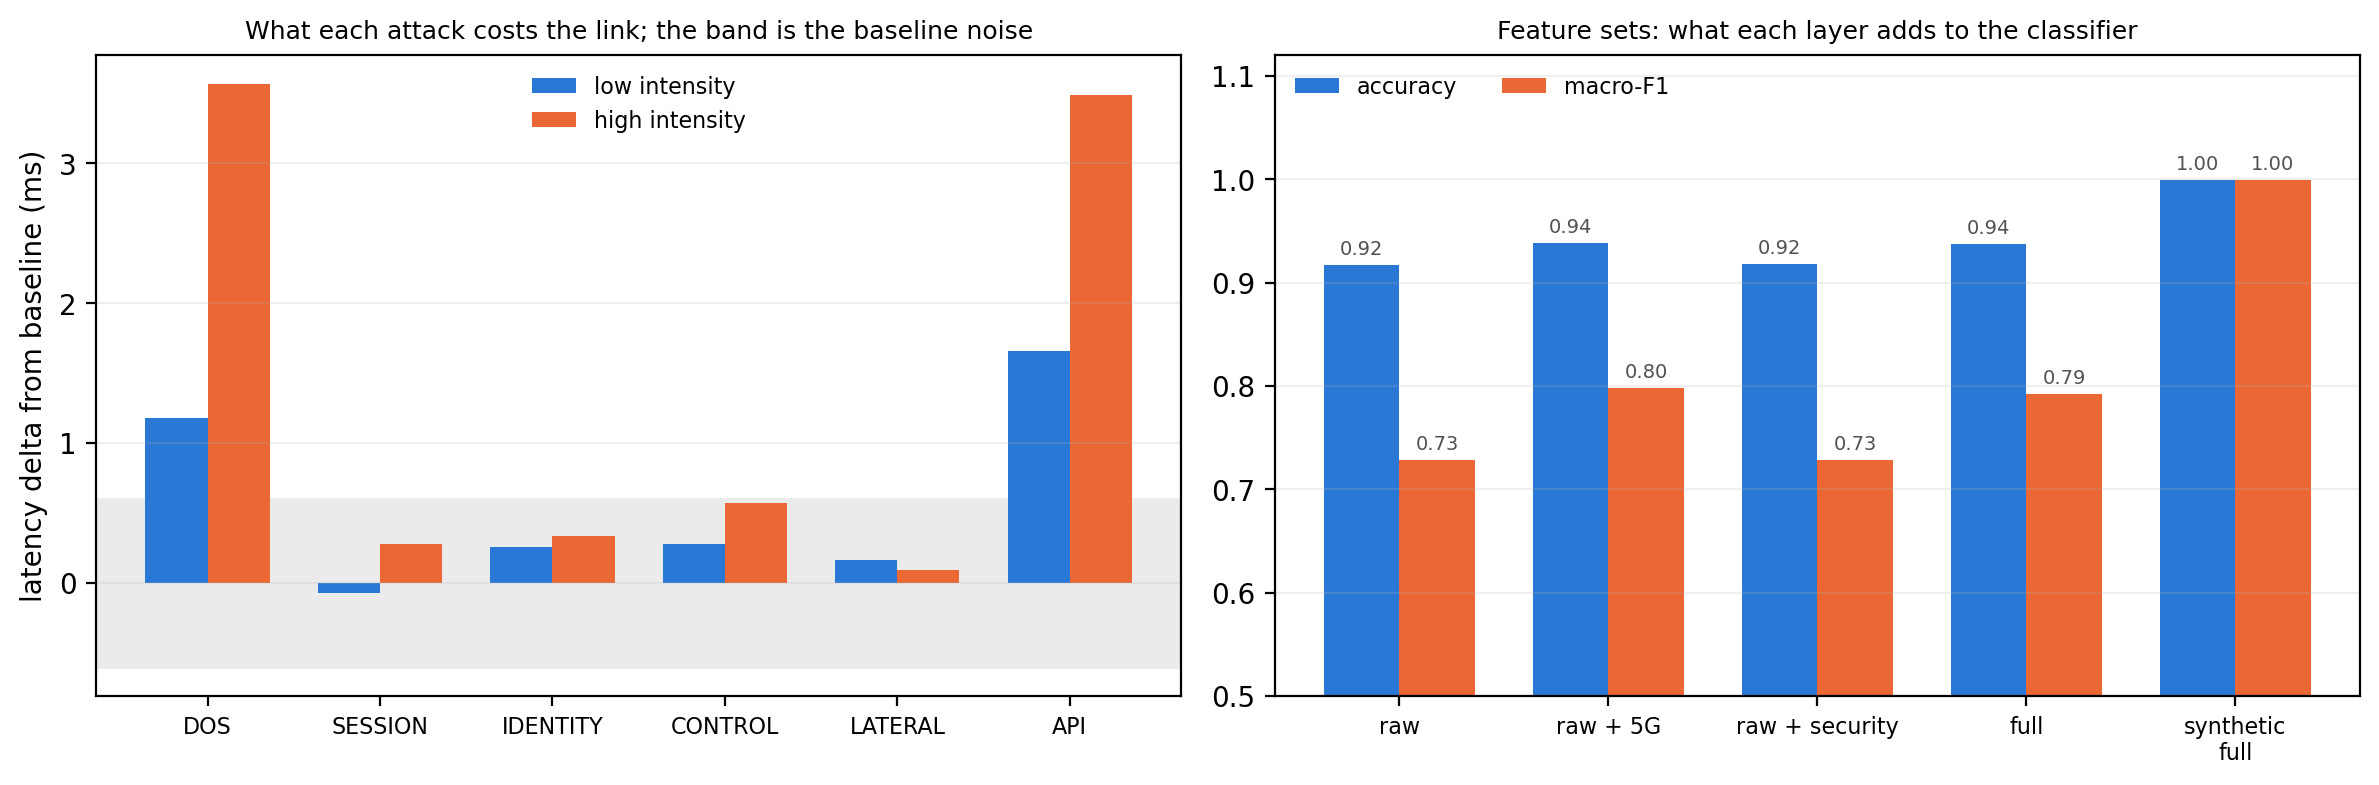
\includegraphics[width=0.56\textwidth]{d2_intensity_features}
\caption{Left: latency cost of each attack at low and high intensity, with the baseline noise band. Right: random-forest accuracy and macro-F1 by feature set.}
\label{fig:model}
\end{figure*}

\paragraph{Setup stage.} Eight runs of 135\,s at 3\,m/s on one cell: a benign
baseline, one suspicious run (failed logins from a misconfigured client) and
one run per attack class, each attack injected in Simu5G between 40 and
80\,s. Every run flew its own mission. The result is a 2,440-row dataset.

\paragraph{Experiment stage.} A 43-run matrix (Table~\ref{tab:matrix})
changes one parameter group at a time from a common baseline: three repeated
baselines with different seeds, then window size, speed, duration, drone
count, cells, slice profile, background load and wireless condition, plus a
hover run; four
suspicious scenario types with two repeats each; and six attack classes at low
and high intensity plus two attack-timing variants. The baseline is the same
135\,s route flight as the setup stage so the datasets stay comparable; the
duration runs patrol the route for 5, 10 and 20 minutes; the multi-drone runs
record one real flight per drone, in sequence, and Simu5G flies the traces
together in one cell 6\,m apart. Every attack is followed by a 10\,s
recovery window labelled suspicious.

\paragraph{Scenarios.} The suspicious runs are degradations with no
attacker: a handover loss spike from two cells at moderate signal, with the
label window placed over the cell boundary the flight plan predicts at
38\,s; a burst of three failed logins per second; a retry storm of 30
unanswered API requests per second; and an eight-second telemetry dropout
produced by pausing the sender. The malicious runs inject one flow per class
into Simu5G from 40 to 80\,s: a UDP flood of 50 or 200 packets per second, a
session hijack reusing the command session from a second address, an
identity theft claiming the drone's identity from another IP and slice,
rogue commands at 5 or 20 per second, lateral movement to an internal
address outside the allowed set, and an application-layer flood of 50 or 200
unanswered API requests per second; the timing variants shorten the flood to
30\,s or split it into three 10\,s bursts. Each manifest states the effect it
expects, a packet rate, a latency shift, loss, a handover or a flag, and the
analysis checks every run against that statement. In total 49 flights were
recorded, and the final dataset holds 17,779 rows: 15,247 normal, 912
suspicious and 1,620 malicious.

\begin{table}[H]
\centering\small
\caption{The experiment run matrix. Baseline: 1 drone, 3\,m/s, 135\,s, 1\,s window, 1 cell, low load, single slice, good signal.}
\label{tab:matrix}
\footnotesize
\begin{tabular}{@{}llr@{}}
\toprule
Group & Variations & Runs \\
\midrule
Baseline & seeds 1, 2, 3 & 3 \\
Window & 0.5\,s, 5\,s & 2 \\
Speed & 1, 8\,m/s patrol & 2 \\
Duration & 5, 10, 20\,min patrol & 3 \\
Drones & 3, 5 & 2 \\
Cells & 2, 3 with X2 handover & 2 \\
Slices & mission+video, three slices & 2 \\
Background load & medium, high & 2 \\
Wireless & moderate, edge of cell & 2 \\
Hover & telemetry and video & 1 \\
Suspicious & handover, auth, retry, dropout $\times$2 & 8 \\
Malicious & 6 classes $\times$ low, high & 12 \\
Attack timing & 30\,s window, three 10\,s bursts & 2 \\
\midrule
Total & & 43 \\
\bottomrule
\end{tabular}
\end{table}

\paragraph{Validation and comparison.} Four checks follow every build. The supplied validator
checks every per-run dataset and every concatenated build for column order,
vocabularies, the signal-quality range and the response mapping. An audit
script recomputes the three behavioural flags of every run from its manifest
and flow contract, independently of the bridge, and counts rows that
disagree. Every run's measured effect is compared with the effect its
manifest declares, such as a packet rate, a latency shift, a handover or a
flag. Finally, three classifiers, a random forest of 200 trees, histogram
gradient boosting and logistic regression behind a standard scaler, are
scored on one stratified 70/30 split with labels and identifiers excluded,
over four feature sets: traffic metrics; traffic plus 5G context (ports,
protocol, slice, cell, signal, handovers); traffic plus security indicators (activity
counts and flags); and the full set, and over the synthetic reference for
comparison.

\section{Results and discussion}

\paragraph{Setup stage.} All eight runs and the concatenated dataset passed
the validator. The baseline model reached accuracy 0.974 and macro-F1 0.931,
against 0.999 on the synthetic reference. On the drone's own flows, only the
two floods measurably slowed the link: DoS added 3.46\,ms and the API flood
3.17\,ms in the attack window, against a noise floor of $\pm$0.7\,ms between
otherwise quiet runs. The other attacks, at 1 to 20 packets per second, were
invisible in timing and detectable only through the behavioural flags and
counts, which is why the dataset carries them.

\paragraph{Validation and expected effects.} All 43 per-run datasets and
the concatenated build passed the validator, and the flag audit reproduced
every behavioural flag from behaviour alone with no mismatches. Every run
showed the effect its manifest expected, and none of the quiet runs raised a
flag (Table~\ref{tab:effects}). The three baselines agree to within 0.3\,ms,
which sets the noise floor. Background load is the largest benign effect,
adding 2.7 and 3.8\,ms with five times the jitter and no flag, the benign
congestion the study needs to separate from attacks; edge-of-cell signal costs
2.0\,ms at $-74$\,dBm against $-56$\,dBm. The two- and three-cell runs record
one and two handovers, the two-cell run also the largest benign loss (7.5\,\%)
at the handover. Three and five drones share the cell without measurable cost.
Among the suspicious runs the handover runs record one handover in the
predeclared window, the auth runs count 120 failed logins, the retry storms
1,195 failed requests, and the dropouts show telemetry activity at zero for
eight seconds; none changes latency beyond the noise. Among the attacks only
the floods lift the latency line (Figure~\ref{fig:panels}); the late rise in
every panel is the descent, not the attack. The rest are seen through
40 session reuses, 40 unusual destinations, 40 and 160 failed identity
attempts, and 335 and 932 command messages against 135 in a baseline.




\paragraph{Parameter sweeps and intensity.} Figure~\ref{fig:sweeps} shows
that speed, duration, drone count, cells and slices leave latency where the
baseline has it, while load and radio condition move it by 2 to 4\,ms, as
much as a high-rate flood. Low
against high intensity separates only the floods (Figure~\ref{fig:model},
left): for session, identity, control and lateral attacks the delay stays
inside the noise band at either intensity, and their intensity shows in the
counts, not the timing. A detector built on latency alone would therefore
confuse a loaded or poorly covered link with a flood, and miss four attack
classes entirely.


\begin{table}[H]
\centering\small
\caption{Measured effect of each scenario on the drone's own flows inside its event window, relative to the three benign baseline runs. $\Delta$L is latency, $\Delta$J jitter.}
\label{tab:effects}
\footnotesize
\setlength{\tabcolsep}{3pt}
\resizebox{\columnwidth}{!}{%
\begin{tabular}{@{}lrrl@{}}
\toprule
Run & $\Delta$L (ms) & $\Delta$J (ms) & Behavioural signal \\
\midrule
Baselines $\times$3 & $\pm$0.25 & $\pm$0.02 & none \\
Load medium / high & +2.7 / +3.8 & +1.4 / +1.3 & none \\
Wireless edge & +2.0 & +0.4 & $-74$\,dBm \\
Cells 2 / 3 & $-0.1$ / $-0.2$ & 0.0 & 1 / 2 handovers \\
Drones 3 / 5 & $-0.6$ / +0.3 & $-0.2$ / +0.2 & 6 / 10 flows \\
S1 handover $\times$2 & +0.3 / +0.2 & +0.3 / +0.1 & 1 handover each \\
S2 auth $\times$2 & 0.0 / $-0.1$ & +0.1 & 120 failed \\
S3 retry $\times$2 & 0.0 / +0.4 & +0.6 & 1,195 failed \\
S4 dropout $\times$2 & -- & -- & telemetry 0, loss 0.5 \\
DoS low / high & +1.2 / +3.6 & +0.3 / +1.3 & burst flag 0 / 40 \\
API low / high & +1.7 / +3.5 & +0.9 / +1.3 & 1,991 / 7,961 failed \\
Session low / high & $-0.1$ / +0.3 & 0.0 / +0.3 & 40 reuses each \\
Identity low / high & +0.3 / +0.3 & +0.1 / +0.2 & 40 / 160 failed \\
Control low / high & +0.3 / +0.6 & +0.2 / +0.7 & 335 / 932 commands \\
Lateral low / high & +0.2 / +0.1 & 0.0 / +0.2 & 40 unusual each \\
DoS 30\,s / bursts & +3.3 / +3.0 & +1.3 / +1.3 & burst flag 30 / 30 \\
\bottomrule
\end{tabular}}
\end{table}

\begin{table}[H]
\centering\small
\caption{Accuracy and macro-F1 by feature set. Traffic metrics are counts, rates, latency, jitter, loss and retransmissions; 5G context adds ports, slice, cell, signal and handovers; security indicators add activity counts and flags.}
\label{tab:model}
\footnotesize
\setlength{\tabcolsep}{2.5pt}
\begin{tabular}{@{}lrrrrrr@{}}
\toprule
& \multicolumn{2}{c}{Forest} & \multicolumn{2}{c}{Boosting} & \multicolumn{2}{c}{Logistic} \\
\cmidrule(lr){2-3}\cmidrule(lr){4-5}\cmidrule(lr){6-7}
Feature set & Acc. & F1 & Acc. & F1 & Acc. & F1 \\
\midrule
Setup stage, all features & 0.974 & 0.931 & -- & -- & -- & -- \\
Traffic metrics only & 0.917 & 0.729 & 0.923 & 0.730 & 0.866 & 0.371 \\
Traffic + 5G context & 0.938 & 0.798 & 0.944 & 0.820 & 0.895 & 0.581 \\
Traffic + security & 0.918 & 0.728 & 0.922 & 0.728 & 0.894 & 0.568 \\
All features & 0.937 & 0.792 & 0.945 & 0.824 & 0.895 & 0.581 \\
Synthetic, all features & 0.999 & 0.999 & 0.998 & 0.998 & 0.991 & 0.988 \\
\bottomrule
\end{tabular}
\end{table}

\paragraph{Models and feature sets.} Table~\ref{tab:model} and
Figure~\ref{fig:model} (right) compare the classifiers on the experiment
dataset and the synthetic reference; the
setup-stage dataset was scored with the random forest only. The two tree
models are close, with gradient boosting slightly ahead on every feature set,
so the ceiling is set by the data rather than the algorithm. Logistic
regression falls far behind, which shows that the suspicious windows cannot
be separated from benign traffic by a linear boundary. For every model the
5G context is the step that matters: slice, cell, ports and signal quality
tell the injected flows apart from the drone's own. The security indicators
add nothing on top of the traffic metrics, because the floods are already
separable by rate and the suspicious rows carry no flags. The random-forest
confusion matrix in the model report confirms where the difficulty lies: about half of the held-out
suspicious rows are recovered and most of the rest fall to normal, the
ambiguity those scenarios were designed to carry.

\paragraph{Realism gaps against the synthetic reference.} The two datasets
share the schema and the direction of every effect but differ in scale. The
synthetic rows carry several times the traffic of the co-simulated ones,
because they aggregate a network segment whereas here each row is one real
telemetry or command stream. Synthetic latency is high and widely spread,
and its malicious rows are slower still; here latency sits near 12\,ms with
little variance and the worst attack adds under 4\,ms, since Simu5G models
one lightly loaded cell with a wired core. Almost every row here has the drone as its source, because only the
radio leg is measured per flow, whereas the synthetic set spreads sources
evenly over drone, core, backend and security monitor. The synthetic set is
also far more balanced across the three labels, since attacks here occupy
only 40\,s of a 135\,s mission, and the optional \texttt{anomaly\_score} is
held at zero. What the co-simulation offers instead is provenance, every
value tracing to a recorded flight and a Simu5G vector, and the honest
difficulty of telling a congested link from an attacked one.

\paragraph{Limitations.} Loss, retransmissions and signal quality are
proxies, taken from the configured send rate, the HARQ error rate and SINR;
authentication status comes from the injected flow's configuration, since
the traffic applications carry no authentication semantics. The classifier
split is over windows rather than whole runs, so the scores are optimistic.
Multi-drone runs were flown one drone at a time, because a second PX4
instance in the same world lost its position estimate. The suspicious class
is the weakest for every classifier, as those scenarios were built to be
ambiguous.

\section{Conclusion}

A Gazebo, PX4, ROS~2 and Simu5G co-simulator was built and used to produce
two validated 44-column cyber-incident telemetry datasets: 2,440 rows from
the eight-run setup stage and 17,779 rows from the 43-run experiment. Every
row traces to a recorded flight and a network
simulation vector, every behavioural flag is reproduced from behaviour with no
mismatches, and every scenario shows the effect its manifest predicted.
Timing alone reveals the two floods and benign congestion; the four low-rate
attack classes need the behavioural indicators. Gradient boosting reaches
macro-F1 0.82, the random forest 0.79 and a linear model 0.58, so the realism
the co-simulation adds lies in suspicious windows no linear boundary
separates. The pipeline is reproducible from the manifests: a scenario is
one YAML file, and the run, validation and comparison follow from it.

\paragraph{Future work.} The natural extension is a ground vehicle working
with the drone over the same network. A UGV added as a second user equipment
on its own recorded trace would let the manifest describe a joint mission,
the drone scouting ahead and the rover following its reported waypoints to
a timed rendezvous. Synchronisation then
becomes measurable as the delay and loss of the coordination flow between
the two vehicles, and the same bridge would emit rows for both on one clock.
New scenarios follow directly: handover of one vehicle while the other
stays, congestion that delays the rover's waypoint updates, and a spoofed
rendezvous command on the coordination channel.

\end{document}
